%% 
%% ACS project dissertation template. 
%% 
%% Currently designed for printing two-sided, but if you prefer to 
%% print single-sided just remove ",twoside,openright" from the 
%% \documentclass[] line below. 
%%
%%
%%   SMH, May 2010. 


\documentclass[a4paper,12pt,twoside,openright]{report}


%%
%% EDIT THE BELOW TO CUSTOMIZE
%%

\def\authorname{David Brazdil\xspace}
\def\authorcollege{Trinity Hall\xspace}
%\def\authoremail{Sarah.Jones@cl.cam.ac.uk}
\def\dissertationtitle{Qishr: Capability-based Protection for the Java Native Interface}
\def\wordcount{14,235}


\usepackage{epsfig,graphicx,parskip,setspace,tabularx,xspace,url,listings,color,paralist}

\newcommand{\reg}[1]{\texttt{\$#1}}
\newcommand{\insn}[1]{\texttt{#1}}
\newcommand{\keyword}[1]{\textsf{#1}}
\newcommand{\class}[1]{\texttt{#1}}
\newcommand{\tool}[1]{\emph{#1}}
\newcommand{\lib}[1]{\tool{lib#1}}


%% START OF DOCUMENT
\begin{document}

\lstset{
	basicstyle=\tt\footnotesize,	% the size of the fonts that are used for the code
	numbers=left,			% where to put the line-numbers
	numberstyle=\footnotesize,	% the size of the fonts that are used for the line-numbers
	stepnumber=1,			% the step between two line-numbers. If it is 1 each line will be numbered
	numbersep=5pt,			% how far the line-numbers are from the code
	backgroundcolor=\color{white},	% choose the background color. You must add \usepackage{color}
	showspaces=false,		% show spaces adding particular underscores
	showstringspaces=false,		% underline spaces within strings
	showtabs=false,			% show tabs within strings adding particular underscores
	frame=leftline,			% adds a frame around the code
	tabsize=2,			% sets default tabsize to 2 spaces
	captionpos=b,			% sets the caption-position to bottom
	breaklines=true,		% sets automatic line breaking
	breakatwhitespace=false,	% sets if automatic breaks should only happen at whitespace
	escapeinside={\%*}{*)},		% if you want to add a comment within your code
	captionpos=t,			% title position
}

%% FRONTMATTER (TITLE PAGE, DECLARATION, ABSTRACT, ETC) 
\pagestyle{empty}
\singlespacing
% title page information
\begin{titlepage} 

\begin{center}
\noindent
\huge
\dissertationtitle \\
\vspace*{\stretch{1}}
\end{center}

\begin{center}
\noindent
\huge
\authorname \\
\Large
Computer Science Tripos, Part III \\
\authorcollege      \\[24pt]

\includegraphics{CUni3.eps}
\end{center}

\vspace{24pt} 

\begin{center}
\noindent
\large

\vspace*{\stretch{1}}
\end{center}

\begin{center}
\noindent
University of Cambridge \\
Computer Laboratory     \\
William Gates Building  \\
15 JJ Thomson Avenue    \\
Cambridge CB3 0FD       \\
{\sc United Kingdom}    \\
\end{center}

%\begin{center}
%\noindent
%Email: \authoremail \\
%\end{center}

\begin{center}
\noindent
\today
\end{center}

\end{titlepage} 

\newpage
\vspace*{\fill}

\onehalfspacing
\newpage
{\Huge \bf Declaration}

\vspace{24pt} 

I \authorname of \authorcollege, being a candidate for the M.Phil in
Advanced Computer Science, hereby declare that this report and the
work described in it are my own work, unaided except as may be
specified below, and that the report does not contain material that
has already been used to any substantial extent for a comparable
purpose.

\vspace{24pt}
Total word count: \wordcount

\vspace{60pt}
\textbf{Signed}: 

\vspace{12pt}
\textbf{Date}:


\vfill

This dissertation is copyright \copyright 2010 \authorname. 
\\
All trademarks used in this dissertation are hereby acknowledged.



\newpage
\vspace*{\fill}

\singlespacing
\newpage
{\Huge \bf Abstract}
\vspace{24pt} 

With the necessity to reuse legacy code, or to employ readily available third-party libraries, it is not uncommon for large applications to be written in more than one programming language. Such heterogeneous environments have inherent advantages, e.g.\ allowing security-critical components to be written in a memory-safe language like Java, while performance-critical code in C, but because there is no runtime separation between the two code bases, it is possible for the native code to corrupt the Java environment or to bypass its security.

Qishr demonstrates that the capability-enabled CHERI processor can be used to isolate Java native code into a safe sandbox, from which it can only interact with the Java runtime and the system kernel through a secure interface. It guarantees that the code cannot break memory safety of Java objects, controls its access to system resources in accordance with the security policy enforced by Java on its classes, and provides a compatibility layer for legacy code written against the standard native interface.

\newpage
\vspace*{\fill}


\pagenumbering{roman}
\setcounter{page}{0}
\pagestyle{plain}
\tableofcontents
% \listoffigures
% \listoftables

\onehalfspacing
\newpage ~ \cleardoublepage % make text start on a fresh double page

%% START OF MAIN TEXT 
\pagenumbering{arabic} 
\setcounter{page}{1} 

\chapter{Introduction}

Writing software in Java and other safe programming languages has inherent advantages, namely the promise of improved robustness, reliability and portability. Yet large software systems are hardly ever written in just one language because there are strong incentives to save money and time by incorporating ready-to-use third-party libraries or legacy code, or to implement some components in a more suitable language, most often in attempt to improve performance. However, the lack of safety makes the so-called \emph{native code} a threat to the Java runtime as it has the potential to compromise its code safety properties and core security mechanisms. The decision to include native code is therefore always a trade-off between security and the benefits it can provide.

According to reports from August 2013, approximately 20\% of the most popular applications on the Google Play store indeed do ship with native libraries~\cite{poeplau2014execute}. Protection of all those applications is more fragile since any bug inside the native code might have much larger repercussions than one contained within the managed portion of the codebase. Worryingly, many critical native code vulnerabilities have been discovered even inside the official Java Development Kit (JDK) framework~\cite{Tan:2008:ESS:1496711.1496736}. 

To the enterprise environment, where security tends to be prioritized, Java is a platform capable of executing untrusted applications inside a safe environment that limits its access to system resources, and even running multiple such applications side-by-side. But the inability to constrain native code in the same manner dictates that only applications written eclusively for the Java Virtual Machine (JVM) can forced to comply with the chosen security policy.

The rest of this dissertation describes Qishr, a prototype JVM extension which explores the potential of using capability-based mechanisms to protect the virtual machines's core from native libraries attached to it via the Java Native Interface (JNI) and their integration into the Java Security Architecture.

\section{Protection with Capabilities}

Capability is a concept of a communicable token which entitles its holder to access a protected resource with a given set of access rights. Security of systems built around this abstraction then rests entirely on the ability to guarantee the unforgeability and integrity of the tokens.

If implemented efficiently, capabilities are a lightweight access control mechanism which offers a natural approach towards least-privilege software compartmentalization~\cite{Watson:2010:CPC:1929820.1929824}, i.e.\ separation of code into smaller security domains with only the rights they necessarily need. Compartmentalization is the key feature as it allows for isolation of untrusted native code, but is also highly desired in general software development because it limits the security risks caused by common bugs.

Most systems implement capabilities in some form, UNIX and its file descriptors are an example of one, but their design is typically not flexible enough to facilitate small-scale software decomposition. Qishr was built for the Capability Hardware Enhanced RISC Instructions (CHERI) platform, an ongoing University of Cambridge research into extending the comodity 64-bit MIPS Instruction Set Architecture (ISA) to support the \emph{object-capability model} directly in hardware. That makes CHERI capabilities not only fast but also highly trustworthy because they are protected on the lowest possible level of the system.

Qishr uses capability compartmentalization to execute untrusted JNI libraries inside a safe sandbox within the JVM process. The native code is given access to a small region of the virtual address space which it can use freely, but its access to system resources and other parts of the address space is controlled. Legacy code can be built against a library which provides a compatibility layer for the standard JNI interface and \lib{c} functions.

Qishr does not guarantee safety of the code inside the sandbox but it does protect the Java runtime from its effects and enforces the same security policy as the Java interpreter. Its proof-of-concept implementation integrates Qishr into JamVM but the design is highly portable to other Java VMs. [MORE]

\chapter{Background} 

% A more extensive coverage of what's required to understand your 
% work. In general you should assume the reader has a good undergraduate 
% degree in computer science, but is not necessarily an expert in 
% the particular area you've been working on. Hence this chapter 
% may need to summarize some ``text book'' material. 
% 
% This is not something you'd normally require in an academic paper, 
% and it may not be appropriate for your particular circumstances. 
% Indeed, in some cases it's possible to cover all of the ``background'' 
% material either in the introduction or at appropriate places in 
% the rest of the dissertation. 

\section{Java Security Architecture}

Java was designed mainly as a universal platform for networked environments which necessarily made its security model one of the most important architectural features. On all its levels, Java addresses the common pitfalls of modern software engineering which can lead to introduction of security vulnerabilities, and thus guarantees a higher minimal level of application robustness and alleviates the process of implementing additional security measures.

At the core of the platform lies the Java programming language, an easy-to-learn type-safe language with automatic memory management, built around the principles of object-oriented programming. These properties significantly reduce the likelihood of writing unsafe code and also encourage the principle of least privilege via separation of executable code and its state into smaller object-level protection domains.

Java applications are expected to be distributed over public networks and therefore the platform has to account for composition of code with varying levels of trust. Untrusted code can be executed inside a safe environment isolated from other code running inside the same virtual machine and be subject to a programmatically managed security policy which can limit its access to guarded resources. This is called the \emph{Java Sandbox Model}.

Additionally, the Java framework provides a large set of extensible security APIs with ready-to-use implementation of many cryptographic algorithms and standardized protocols for public key infrastructure, authorization and encrypted network communication. 

\subsection{Code Safety}

The security of the Java platform is deeply rooted in the type, memory and control flow safety properties of its executable code. The language and the instruction set were crafted in a way that program bugs are likely to be caught by the compiler and pre-execution bytecode verifier, and other will raise exceptions at runtime. 

Java's type system is dynamic, although most types are actually checked statically for the sake of performance. Operations which are checked at runtime include array assignments, operations on generic classes and type casts. Unfortunately, the type inference algorithm has been shown to contain vulnerabilities~\cite{Suenaga:2012:JavaVulnerability} which make way to type confusion attacks~\cite{Oh:2012:JavaExploitReport} and these can subsequently be exploited to bypasss the security of the platform~\cite{McGraw:1999:SJG:298616}.

Memory safety in Java is strongly connected to the principles of OOP. Code does not have direct access to the heap but rather has to adhere to a model of a memory space structured into object instances and their internal fields protected by the reference monitor, accessed through opaque references and automatically managed by the garbage collector. Together with the type system and explicit range checks, Java prevents common bugs, e.g.\ buffer overflow or dangling pointers, which can give the attacker access to an arbitrary part of the memory.

\subsection{Object Encapsulation}

The assurances described above are the cornerstone of the Java security as they allow for isolation of individual software modules by enabling them to encapsulate their state. 

Individual classes are separate protection domains which only permit the modification of their inner state through a set of transactions exposed in their public interface. These methods become the only entry points into the respective protection domain and can be used by the object to control access to its state and to prevent operations which could leave the state inconsistent.

% --- REMOVED ---
% Limiting the scope of the code which can access the state also makes it possible to argue about the high-level security properties of an object class. As the authors of Joe-E [REF] point out, however, Java still contains language features which can prevent such reasoning and suggest building a more secure platform around its safe subset.

\subsection{Java Sandbox Model}

The design of the Java platform was deeply influenced by the web and the need to dynamically load executable code from various, potentially untrusted sources into one instance of the Java virtual machine. The language safety properties do protect the integrity of the memory, but just by themselves cannot prevent the external code from abusing the system resources available to the VM or interacting with code from a different source. To this end, the platform provides a number of access control mechanisms which make it possible to execute differents portions of the loaded code with different sets of permissions available to them. 

\begin{figure}
	\centering
	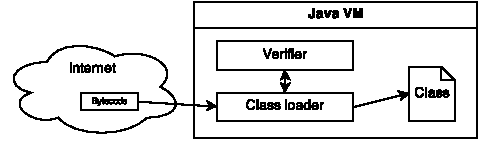
\includegraphics[width=0.8\textwidth]{dia_java_classload.pdf}
	\caption{Class loading in Java}
\end{figure}

Java code is loaded into the virtual machine by a special objects called class loaders. The main task of a class loader is extracting bytecode from some external source and passing it on to the bytecode verifier which determines whether it complies with the required language safety properties. Typically it also selects the desired security policy which will be later enforced upon it, and it is the class loader's task to make sure that the newly loaded code will not replace any existing classes (including itself and other security-critical classes) unless this is explicitly allowed. 

Every Java VM provides a simple "primordial" class loader implemented in native code which bootstraps the framework and immediately hands the process over to its loader. Code with sufficient permissions can then define new, potentially simultaneosly active class loaders and arrange them into hierarchies. Since class loaders are also responsible for resolving classes and methods for the code loaded by them, they can be used to create local namespaces, effectively isolating codebases which should not be allowed to interact.

The last component of the Java sandbox is a reference monitor, called the security manager. Before untrusted code is called, the parent can set a thread-local reference to a \class{SecurityManager} object which implements the security policy that is to be enforced. Should the untrusted code attempt to access system or VM resources during its execution, it must do so through the framework API and these methods always consult the active Security Manager before access is granted.

\subsection{Java Native Interface}

Just like bytecode, shared libraries are loaded by a class loader and reside in its namespace. The method resolver then uses a naming convention defined in the JNI specification to bind a Java method (marked \keyword{native}) with a corresponding function in the native library.

\begin{figure}
	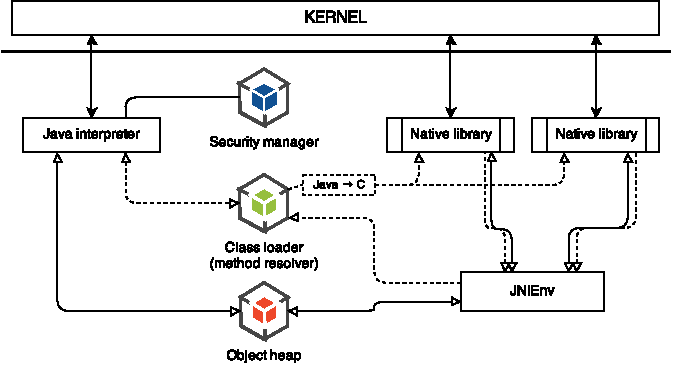
\includegraphics[width=\textwidth]{dia_jni_orig.pdf}
	\caption{Schematic diagram of the core JVM security components with respect to native code. Solid lines represent data flow paths, dashed lines show control flow. [TODO: draw threats in red?]}
	\label{fig:OverviewJNI}
\end{figure}

\begin{figure}[t]
	\lstinputlisting[language=Java,title=HelloJNI.java]{example/HelloJNI.java}
	\lstinputlisting[language=C,title=HelloJNI.c]{example/HelloJNI.c}
	\caption{Example of a method implemented with JNI. \texttt{getMessage} calls \texttt{NewStringUTF} which instantiates a new \texttt{String} object and returns its reference to the caller.}
	\label{listing:HelloJNI}
\end{figure}

Developers are provided with a C/C++ header which contains the definitions of types compatible with the primitive types used in Java, the \texttt{jobject} type to represent object references (typically pointers to the object heap) and the \texttt{JNIEnv} data structure containing functions that provide an API for interfacing with the VM, such as reading/assigning values of object fields, creating new objects, or invoking other managed methods. A pointer to an instance of \texttt{JNIEnv} is passed to the function together with the actual parameters of the corresponding method call. Figure~\ref{fig:OverviewJNI} gives a simplified overview of the architecture, and Figure~\ref{listing:HelloJNI} shows an example of a simple Java class with a \texttt{native} method implemented in C.

However, the Java platform does not provide any means of containing native code. Because it resides in the same virtual address space as the VM, it does have unlimited access to the object heap and can both read and modify any object data on it, including the class loaders. Similarly, native code can perform system calls without the knowledge of the security manager or even modify the state of the virtual machine. Giving a piece of code the permission to load native libraries is therefore equivalent to giving it all the permissions as well as unlimited access to the VM state.

\subsection{Trust and Native Code}

Previous sections have explained the role of the three pillars of Java security: language safety, secure class loading and a reference monitor. To understand how native code fits into this picture, it is essential to understand the relationship between these three components and the assumptions they make.

A Java VM consists mainly of a bytecode interpreter (or a compiler into native code), a minimal class manager with a bytecode verifier, memory management code and a small set of low-level classes implemented in native code which faciliate communication between the VM and the managed code, e.g. to provide reflection. The entire VM codebase must be fully trusted and it must ensure that only safe code will ever be executed.

The framework, on the other hand, is mostly written in Java with a relatively small number of native methods which give managed code access to system calls and only these therefore need to be trusted to not violate language safety. The framework includes classes which abstract over the system resources, provides its own class loader, which selects the appropriate security policy and passes bytecode over to the VM's verifier and loader, and a default implementation of the security manager. All of these Java classes, as well as the native code, are trusted to not compromise the class hierarchy and to always enforce the active security policy.

Since both the developers of the virtual machine and the system administrator have all of the code above under control, trusting it is not a problem. However, when it comes to application code, we immediately see a big discrepancy between programs written purely in Java and those which ship with native libraries. Even if a Java application is not fully trusted, activating the security manager enables the administrator to ensure the safety of its execution. On the other hand, any application with native code must be fully trusted as its safe execution cannot be guaranteed.

\section{Security with Capabilities}

Memory protection and decomposition of software into isolated components are highly desired security properties but contemporary computer systems do not provide the means of achieving them. Most commonly, operating systems provide controlled process isolation with virtual addressing and inter-process communication. This approach, however, suffers from poor scalability due to a high performance penalty imposed by the Translation Look-aside Buffer (TLB) as the number of protection domains and the domain switches between them increases~\cite{watson2012cheri}.

Conversely, capabilities have proven to be a security primitive which allows for fine-grained memory protection and low-overhead software compartmentalization within a single address space. This makes them an ideal tool for applying the principle of least privilege on a very small scale, i.e. running each software component with only the access rights it needs, and that in turn mitigates the consequences of security vulnerabilities which inevitably appear in the code. 

\subsection{Overview of CHERI}

The CHERI extension of the MIPS ISA adds capabilities as a new security primitive that can be utilized by the operating system and other software running on top of it. The result is a hybrid capability architecture which is backwards-compatible with the traditional form of process isolation with virtual address spaces, but simultaneously enables capability-aware software to employ additional security measures within the address space assigned to the running process.

Applications can use CHERI capabilities in many ways. The most elementary use case is treating them as fat pointers~\cite{kwon2013low}, i.e.\ pointers with an upper limit and a set of permissions. This is particularly useful when dealing with pointers to arrays or data structures as the hardware automatically performs zero-overhead runtime bounds checking and thus prevents exploitation of buffer overflow bugs. 

CHERI capabilities can also be sealed, in which case they cannot be used in load/store instructions any more and become pure tokens of authority exchanged between the components. These are the underlying support for the idea of implementing protection domains with \emph{object capabilities}. An object capability consists of a pair of sealed capabilities: 
\begin{inparaenum}[\itshape a\upshape)]
\item a memory region designated to the object with a pointer to an entry function (\emph{code capability}), and
\item a protected argument (\emph{data capability}).
\end{inparaenum}
Each such pair of compatible capabilities can be used by the holder to perform an atomic domain transition with the \insn{CCall} instruction which unseals the two capabilities, sets the limits of accessible memory and jumps to the given function. Object capabilities can therefore be safely passed to an untrusted component (if confined to a non-overlapping memory region) as they only allow access to the internal state of the object via controlled access points. It is easy to see that a similar principle lies at the heart of the object paradigm implemented by Java and other object-oriented languages.

One of the weaknesses typically associated with capabilities is the difficulty of access rights' revocation, e.g.\ after an object is destroyed and its memory region allocated to another. CHERI does not solve this problem entirely and still relies on the software stack to either guarantee virtual space non-reuse or to provide a form of capability garbage collection. It does, however, alleviate the process by enabling capabilities to be marked \emph{ephemeral} and the right to store ephemeral capabilities to be removed from a majority of an object's memory space, hence bounding their potential spread.

\subsection{Protecting Capabilities}

CHERI implements capabilities as 4-word (256-bit) data structures with the following fields:
\begin{description}
	\item[Base \& length] A pointer to the base of the memory region and its length; both 64-bit values.
	\item[Permissions] 31-bit mask which describes the operations that may be performed with the capability.
	\item[Unsealed bit] If this flag is set, the capability can be used in general-purpose capability operations.
	\item[Object type] A 64-bit identificator to ensure that only corresponding code and data capabilities are used together.
\end{description}

Because these are too big to fit into standard registers, CHERI extends the register file with 28 general-purpose and five specialized capability registers, and defines their function in a new ABI convention. Extra caution is required when calling less trusted code because it may not conform to the convention. Specifically, the caller must explicitly clear all unused registers to avoid leaking rights and private data to the callee.

Capabilities must be protected by the hardware yet at the same time it is highly desirable to allow capabilities to be stored together with normal data. To this end, each capability register has a tag which indicates whether it is holding a valid capability or not, and correspondingly the physical memory is required to associate a tag with every fourth word (capabilities in memory must be aligned accordingly). The instructions defined in the extended ISA are then the only ones allowed to set this tag as they are trusted to preserve the security properties, mainly that capability manipulation must never increase rights. Storing into memory with original MIPS instructions always clears the tag of the corresponding capability block. Invoking a capability instruction with an invalid argument traps.

\subsection{Pointer Indirection}

As mentioned earlier, one of the prerequisities of successful compartmentalization of native code is the ability to prevent a component from accessing addresses beyond the region of the virtual address space designated to it. But at the same time, it is important that such containment is seamless in order to retain the ability to run legacy code.

The solution adopted in CHERI is based on pointer indirection, where addresses of all non-capability loads and stores are treated relative to a capability that the active domain carries in register \reg{C0}. Normal pointer to address \texttt{x} then always translates to \texttt{\reg{C0}.base~+~x} and a memory access instruction will trap if \texttt{x~>=~\reg{C0}.length}. 

\reg{C0} initially contains the capability to the entire virtual address space but a less trusted component can be invoked with a capability granting access only to its subset, effectively denying the component access to the rest of the address space without breaking any of its internal pointer arithmetic.

The same principle is applied to instruction fetch from \reg{PC}, only it is indirected through \reg{PCC} which can only be set by the \insn{CCall} instruction.

\subsection{Object Capabilities}

As mentioned before, object capabilities are formed by a pair of sealed capabilities. The object owner first creates an unsealed capability with \emph{seal} and \emph{execute} rights such that the capability's type is a pointer to the entry function relative to the region defined by the base and length, i.e. \texttt{base~+~type~=~\&function} and \texttt{type~<=~length}. Notice that only code which already has the rights to the memory containing the entry function can create this capability. 

The capability is then sealed with the \insn{CSealCode} instruction, becoming the code capability of the object, and is used once more in \insn{CSealData} to seal an arbitrary capability defining the address space of the object. Both components inherit the \emph{object type} field from the unsealed capability.

When a valid object capability pair is passed to the \insn{CCall} instruction, the unsealed code capability becomes the new value of \reg{PCC}, its type is assigned to \reg{PC} and the unsealed data capability is stored in \reg{IDC} (\texttt{=\reg{C27}}). Typically, the entry function should begin by copying the capability from \reg{IDC} to \reg{C0} as \reg{C0} would have been cleared by the caller.

Additionally, \insn{CCall} pushes the old values of \texttt{\reg{PC}~+~4}, \reg{SP}, \reg{PCC} and \reg{IDC} onto a trusted system stack, from which they are restored once the callee invokes \insn{CReturn}.

\subsection{Multithreading}

One of the prevailing limitations of the CHERI prototype is that the trusted thread stack capability is not thread-local and hence it is not safe to perform multiple object calls simultaneously. 

For this reason, the host is currently forced to acquire a (reentrant) lock before it invokes an object capability. Multithreaded access to the sandbox is also not discussed in this dissertation and its implications on the protection mechanisms would require very careful and detailed consideration.

\chapter{Related Work} 

This chapter covers relevant (and typically, recent) research 
which you build upon (or improve upon). There are two complementary 
goals for this chapter: 
\begin{enumerate} 
  \item to show that you know and understand the state of the art; and 
  \item to put your work in context
\end{enumerate} 

Ideally you can tackle both together by providing a critique of
related work, and describing what is insufficient (and how you do
better!)

The related work chapter should usually come either near the front or
near the back of the dissertation. The advantage of the former is that
you get to build the argument for why your work is important before
presenting your solution(s) in later chapters; the advantage of the
latter is that don't have to forward reference to your solution too
much. The correct choice will depend on what you're writing up, and
your own personal preference.

\section{Joe-E}

\section{Dalvik}

sandbox by linux uid

\section{SafeJNI}

\section{Robusta}

doesn't support dynamic loading (and by design cannot)

\section{Capsicum}

\chapter{Design and Implementation} 

A proof-of-concept implementation is based on JamVM~[REF], a highly-portable and compact Java virtual machine, the GNU Classpath framework~[REF] and is comprised of XXX lines of C and XXX lines of MIPS assembly. The sandboxing code resides entirely in the virtual machine's codebase and therefore other frameworks, such as OpenJDK~[REF], Apache Harmony~[REF] or the Android framework~[REF], could just as easily be used instead.

\begin{figure}
	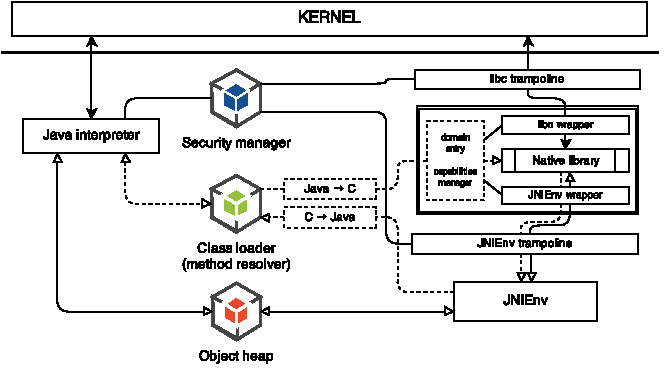
\includegraphics[width=\textwidth]{dia_jni_caps.pdf}
	\caption{Diagram of a Java VM running a native library in a CHERI sandbox. All references are passed across the domain boundary as capabilities.}
	\label{fig:OverviewCheriJNI}
\end{figure}

An overview of the modified design is given in Figure~\ref{fig:OverviewCheriJNI}. As opposed to the the original schematic in Figure~\ref{fig:OverviewJNI}, the native library is now fully contained inside a CHERI sandbox that limits its memory access to a designated region of the virtual address space, thus preventing it from reading or modifying the state of other components. The code is not allowed to perform system calls and similarly cannot directly interact with the VM. Its only option is to invoke a trampoline function inside the host domain which performs the operation on the native code's behalf provided that it is not in conflict with the currently active security policy.

In order to retain source-level backwards compatibility, the native code can be compiled against \lib{qishr} which provides wrappers for \lib{c} functions and the \texttt{JNIEnv} interface, and also automatically manages the capabilities passed to the sandbox, allowing for seamless integration of legacy code into the sandboxed environment.

\section{Porting Java to CHERI}

Even though the MIPS64 architecture, which CHERI extends, has been around for a while~[REF], processors implementing its instruction set are yet to penetrate the consumer electronics market~[REF]. Software support for this architecture therefore still remains quite rare and its lack proved to be one of the obstacles in the early stages of this project as virtual machines always rely on at least some small amount of assembly code, typically more if optimized for performance. Likewise, the choice of the VM was limited by the fact that the only operating system ported to CHERI to date is FreeBSD, and the only compiler capable of producing CHERI code is LLVM/Clang. 

Initially, efforts were invested into porting a minimal subset of the Android runtime, ideally the emerging LLVM-based ahead-of-time ART compiler~[REF] which will replace the original Dalvik VM in the future releases of Android. Porting ART to CHERI is especially attractive because it translates Dalvik bytecode (equivalent to Java bytecode) directly to native code optimized for running on resource-restricted platforms much like the CHERI prototype. Being based on LLVM, ART could also use the CHERI back-end in order to embrace the security enhancements offered by capabilities while running managed code.

The tight integration of ART (and its numerous dependencies) to a specific platform and toolchain does, however, make porting it to another substrate a very time-consuming task. The obstacles of replacing GCC with LLVM/Clang in the Android build system have mostly been solved by Linaro~[REF], and ART's pre-existing MIPS32 support and LLVM nature therefore should have made emitting MIPS64/CHERI instructions a straightforward extension. Sadly, fixing its codebase, abundant in Linux-specific code and pointer arithmetic assuming 32-bit pointer length, is far beyond the time frame of this project.

After a brief period of experimentation with other Java virtual machines suitable for the embedded environment, the combination of JamVM and GNU Classpath framework was selected for its:
\begin{itemize}
\item complete implementation of the JVM and JNI specifications (versions~5 and 1.4 respectively)
\item strict compliance with POSIX standards
\item minimum amount of platform-specific code
\item overall simplicity of the codebase
\end{itemize}
The price is that JamVM is merely a Java interpreter and thus is unlikely to see a non-negligible performance gain from optimizations which could be achieved with the CHERI ISA, namely hardware bounds checking (a common Java bottleneck~[REF]).

\section{Library Loading}

The process of loading a native library is initiated by calling the \texttt{loadLibrary} method of the \class{System} class. The VM looks for a shared object file of the given name inside lookup folders and attempts to load it with the mechanism approprite fors that platform, e.g.\ \lib{dl} on variants of UNIX. When running on CHERI, this mechanism is now defined to be \lib{cheri} -- a library the CHERI SDK provides for managing sandbox instances. 

\begin{table}
	\centering
	\begin{tabular}{|c|c|c|}
		\hline
		\textbf{Start addr}	& \textbf{Purpose} 				& \textbf{Access rights} 	\\
		\hline
		0x0000				& guard page 					& no access								\\
		0x1000				& metadata 						& read only								\\
		0x2000				& guard page 					& no access								\\
		0x8000				& sandbox image					& read/write 							\\
		J + 0x0000			& guard page 					& no access								\\
		J + 0x1000			& heap							& read/write							\\
		K - 0x1000			& guard page					& no access								\\
		K + 0x0000			& stack							& read/write							\\
		\hline
	\end{tabular}
	\caption{Address space layout of a sandbox instance from the point of view of the sandboxed code. \texttt{J} is the first page-aligned address such that the sandbox image fits between \texttt{0x8000} and \texttt{J}. \texttt{K} is equal to the end of the address space minus the size of the stack.}
	\label{table:addressSpaceLayout}
\end{table}

\lib{cheri} starts with reserving a memory region for the newly created sandbox, preparing the guest's address space layout as summarized in Table~\ref{table:addressSpaceLayout} and memory mapping the \emph{sandbox image} (library object file) into that region. If successful, it returns two object capabilities. One object represents the sandbox domain, with both the code and data component equal to the designated memory space and the entry point at \texttt{0x8000} as dictated by the CHERI ABI. 

\label{sec:SystemObject}
The other is a system object which the sandbox can use to invoke a method inside the host domain. Its code component is the entire address space of the process, with an entry function inside \lib{cheri} which sets up the capability registers and hands over to a function selected by the host. In order to enable it to identify the domain it was invoked from, the data capability is set to the memory region of the sandbox. The entry function therefore does not set \reg{C0} from the data component but rather from the code capability of the object.

This mechanims is sound and works well for simple examples, but it is still quite undeveloped. The sandbox image must be a statically linked binary stripped off any relocation and symbol information -- so it can be directly mapped to memory -- and have the entry point at a fixed offset. This currently makes it equivalent to Robusta. Conceptually, however, there is no reason why dynamically linked code could not be loaded into the sandbox. As the platform matures, it should therefore become possible to sandbox shared libraries without having to relink or strip them first.

\section{Method Binding}

\subsection{Resolution}

JNI defines a naming convention which encodes the class name, the method name and also its signature into the name of the native symbol that the class loader searches for in the loaded shared libraries. Unfortunately, the fact that CHERI sandbox images currently cannot contain symbol information makes this process more complicated.

For the time being, Qishr uses a simple workaround. When the entry function is invoked with \emph{operation code} \texttt{1} (passed to it in \reg{a0}), the sandbox should extract a function name string from a read-only capability in \reg{C1} and look it up in its own symbol table. If found, it should return a non-zero handle, otherwise it should return \texttt{NULL}. The implementation in \lib{qishr} will look for the symbol in a list of function name and pointer pairs pregenerated by the \tool{Ctags}\footnote{\url{http://ctags.sourceforge.net/}} code analyzer and a provided script. The handle is therefore the pointer to the function relative to the base of the inner address space.

\subsection{Invocation}

Operation code \texttt{2} is designated for method invocation. The host calls the sandbox object with the handle of the native method it previously acquired in \reg{a1}, the method's signature as a string in \reg{C1} and the actual parameters in the remaining registers. Primitive arguments are stored in the standard MIPS registers and Java objects as sealed capabilities (\S\ref{sec:MemorySafety}) in the capability registers. Respectively, registers \reg{v0} and \reg{C3} are to be used by the sandbox for the return value.

The number of arguments is currently limited to 6 primitives and 6 objects which is enough for most practical purposes, but the JNI specification allows functions to have up to 255 arguments of any type. A straightforward solution would be to reserve one of the capability registers to pass in a pointer to a buffer containing the arguments which did not fit into registers, much like the MIPS ABI which stores first four arguments in registers and the remainder on the stack.

\lib{qishr}'s entry function implementation stores the capabilities to Java objects in its capability manager (\S\ref{sec:CapabilityManager}) and replaces them with pointers to its internal object heap. It then scans the method's signature so as to correctly order the arguments and invokes the function at the given address (it trusts the host to pass it a valid handler) according to the MIPS N64 ABI convention. If the return value is a Java object, the internal pointer is first replaced by the corresponding capability retrieved from the capability manager.

\subsection{Trap Handling}

At the time of writing, Qishr does not handle the situation when the sandboxed code causes a capability-related exception, such as violating the permissions or length. Until very recently, the operating system would handle CHERI traps simply by setting \reg{v0} to negative one, \reg{v1} to the error code and returning to the most recent caller (popping the trusted stack). Because this does not allow the caller to reliably distinguish a successful call from an erroneous one, it has been replaced with sending a UNIX signal to the process without popping, i.e.\ to the active sandbox. 

The sandboxed code could embrace this mechanism to recover from traps and to throw appropriate Java exceptions. It would, however, be necessary to further consider how the host could recognize an unhandled trap... [ TODO ]

\section{Interaction with the VM}

The \texttt{JNIEnv} data structure, which each native method receives as its first argument, is the main communication gateway between native code and the managed environment. But because its designers assumed that native code can bypass it any way, it completely lacks any form of protection against misbehaving code. With the native code sandboxed, a \texttt{JNIEnv}-like interface can be the only channel between the sandbox and the VM core, and protecting the core's integrity in the presence of untrusted code becomes worthwhile.

This interface is implemented using the system object capability (\S\ref{sec:SystemObject}) which invokes a \texttt{JNIEnv} trampoline in the system domain. The calling convention again assumes that the first primitive argument is the operation code and the remaining registers are used for the actual parameters of the operation. Most of the operations retain the same semantics as their original counterparts, and will simply delegate the call to the corresponding \texttt{JNIEnv} function after the correctness of the arguments is verified. 

Legacy code compiled against \lib{qishr} is provided with a wrapper which automatically translates \texttt{JNIEnv} invocations to \insn{CCall}s into the host domain.

\subsection{Native Handles}
\label{sec:MemorySafety}
\label{sec:CapabilityManager}

\begin{figure}[t]
	\begin{lstlisting}[language=C]
jobject point;

// ...

jclass clazz = (*env)->FindClass(env, "java/awt/Point");
if (clazz == NULL) { /* class not found */ }

jfieldID fid = (*env)->GetFieldID(env, clazz, "x", "I");
if (fid == NULL) { /* field not found */ }

(*env)->SetIntField(env, point, fid, 1234);
	\end{lstlisting}
	\caption{JNI code setting the value of a public field.}
	\label{listing:SetFieldValue}
\end{figure}

In order to interact with the runtime class hierarchy and the internals of Java objects, native code must first request handlers to these elements, namely class objects, method identifiers and field identifiers, which it later uses in \texttt{JNIEnv} calls. Figure~\ref{listing:SetFieldValue} shows an example of such call, acquiring the handle to the \class{Point} class, its \keyword{public} field \texttt{x} and assigning it an integer value.

access control

\subsection{Object References}

\subsection{Garbage Collection}

\subsection{Array Operations}

\subsection{Direct Buffers}
\label{sec:DirectBuffers}

\subsection{State Consistency}

\section{System Calls}

all Java domains - language safety, security policies

VM domain remains the only one that can do system calls => GNU Classpath now provides services around system calls but those must go through the trusted trampoline

\subsection{Threads}

\chapter{Evaluation} 

% For any practical projects, you should almost certainly have some kind of evaluation, and it's often useful to separate this out into its own chapter. 

\begin{figure}
	\centering
	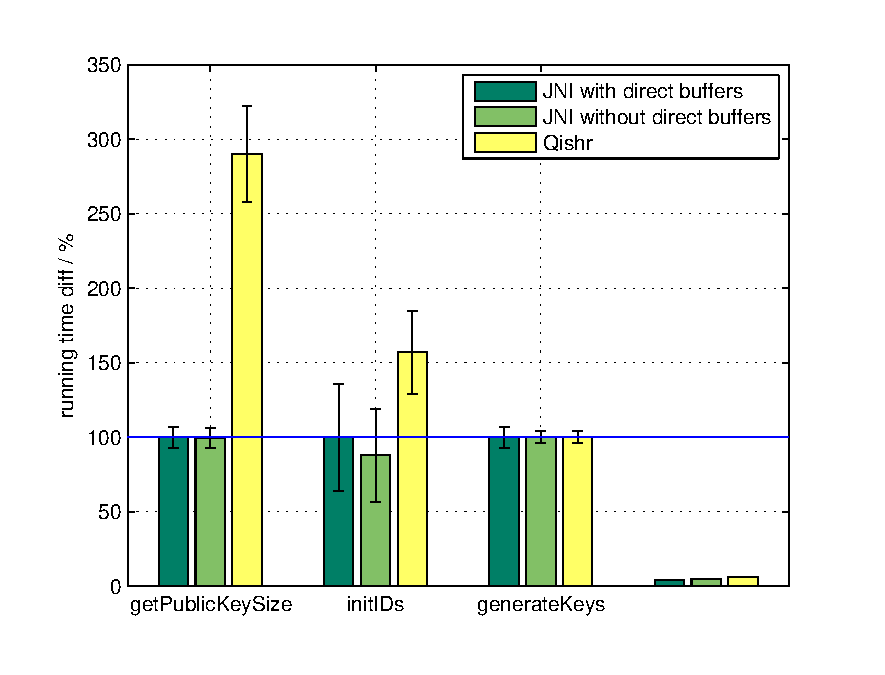
\includegraphics[width=0.8\textwidth]{chart_overhead.eps}
	\caption{Performance overhead of Qishr.}
\end{figure}

\chapter{Summary and Conclusions} 

As you might imagine: summarizes the dissertation, and draws 
any conclusions. Depending on the length of your work, and 
how well you write, you may not need a summary here. 

You will generally want to draw some conclusions, and point
to potential future work. 




\appendix
\singlespacing

\bibliographystyle{unsrt} 
\bibliography{acs-dissertation} 

\end{document}
